\chapter{Detecção de Intrusão em um Cenário Real} \label{ch:cenário-real}
 %- Em cada capitulo adicionar um texto introdutório

Este capítulo esta organizado da seguinte forma: A próxima seção apresenta o cenário de testes, descrevendo características gerais da rede selecionada para os teste. Na seção \ref{sec:infraestrutura} será abordado a infraestrutura usada para os testes, ferramentas utilizadas e as configurações feitas. Na seção \ref{sec:testes} será descrito os testes realizados com suas respectivas justificativas. Na seção \ref{sec:resultados} será apresentado os resultados esperados e obtidos, problemas encontrados e a comparação das ferramentas e por último, na seção \ref{sec:conclusão}, uma breve conclusão.

 \section{Metodologia dos Testes}
 % (Adicionar o escopo dos testes): descrever o ambientes,
 \subsection{Cenário de Testes} \label{sec:cenário}
 %Descrever o cenário. Ex: Uma rede com XXX usuários; Os usuários utilizam
 %diferentes ferramentas,...
 %Adicionar gráficos de utilização da rede

 A rede selecionada para ser monitorada tem os valores especificados na tabela. Podemos verificar que em um determinado período do dia o pico de trafego chega a 107,25 Mbps, valores considerados ideais para o experimento, inclusive para tentar validar os recursos alocados. 

 Em um primeiro momento, selecionou-se uma rede

 \subsection{Infraestrutura Definida para Testes} \label{sec:infraestrutura}
 %Descrever o que foi utilizado:
 %Ex: Equipamentos - Servidores, ....
 %    Configuração
 %    Ferramentas - Snort (referenciar capítulo), ...

 No ambiente de teste foi usado uma máquina Dell com 134 Megabytes (MB) de memória RAM e 40 núcleos. Usou-se XenServer \cite{xenserver} versão 7, sistema operacional (SO) \textit{opensource} da Citrix voltado para virtualização. Foram testados outros SOs porém somente o XenServer possuía, na época da instalação do ambiente, \textit{firmware} da placa de rede do \textit{host} compatível e que funcionava com instabilidade. 
 
Outro fator que pesou na escolha do SO foi a experiência com a plataforma e por existir uma interface para gerencia chamada XenCenter que roda no Windows. Uma alternativa \textit{opensource} desse software é o OpenXenManager que funciona nos sistemas Unix \cite{openxenmanager}.

No primeiro momento, foi instalado uma máquina virtual com o sistema operacional Debian 9.3 \textit{codename} Wheezy \cite{debianwheezy}, uma distribuição linux com uma proposta de ser totalmente livre, usada como base para instalação de outras máquinas utilizando o recurso de \textit{snapshot}, uma cópia de uma máquina virtual rodando em um certo momento, do XenServer. O uso desse recurso foi necessário para criar um ambiente igual para os IDSs.

Foi alocado 8 MB memória RAM, 4 processadores e 100 Gigabytes(GB) de espaço em disco para o \textit{snapshot}. Esses valores foram definidos com base em um estudo \cite{mikelococo} que considerava vários fatores, como largura da rede, localização do IDS e versão, tipo do capturador de tráfego e tamanho da base de assinaturas para dimensionar os recursos de memória e processamento, aplicado especificamente ao Snort. A mesma regra foi aplicada ao Suricata.

Para o \textit{host} conseguir pegar o pacotes destinados a rede escolhida para ser monitorada foi necessário uma configuração de espelhamento no roteador B (Figura \ref{fig:infra-ambiente}) que consiste na copia dos pacotes que saem pela porta dessa rede no roteador para a porta conectada no \textit{host} que possui uma largura de banda de 10 Gigabits. A interface de rede do \textit{host} precisou ser configurada no modo \textit{promisc}.

Posteriormente criou-se quatro máquinas virtuais, duas usadas para instalação dos IDSs (Suricata e Snort) e a terceira para instalação das ferramentas usadas para simular ataques a rede. Optou-se pela instalação do sistema Kali Linux \cite{kalilinux} para geração de ataques pois nele existe várias ferramentas nativas para testes de penetração e auditoria de segurança (Metasploit \autoref{sec:metasploit} e NMAP \autoref{sec:nmap}). 

Na quarta máquina foi instalado o \textit{framework} Pytbull (\autoref{sec:pytbull}), ela servirá também como alvo das simulações dos ataques. A infraestrutura final pode ser visualizada na \autoref{fig:infra-ambiente}.

 \begin{figure}[!htb]
  \centering
  \caption{Infraestrutura do ambiente de teste}
  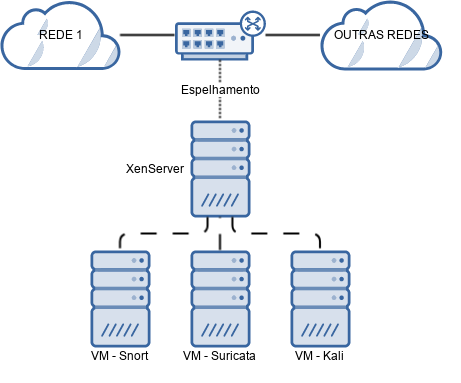
\includegraphics[scale=.65]{infra.png}
  \label{fig:infra-ambiente}
  \legend{Fonte: Autoria própria}
 \end{figure}

Para coleta das informações de uso de recurso de hardware como memória, processamento e I/O das máquinas com os IDSs foi utilizado o \textit{daemon} Collectd \cite{collectd}. Outra opção para esse finalidade é a utilização de um servidor de monitoramento como o Zabbix \cite{zabbix}. A ideia de ter duas ferramentas para essa analise é fazer um comparativo e validar as informações coletadas.

O formato usado para facilitar a análise do \textit{logs} foi JavaScript Object Notation (JSON), um formato simples, leve e de fácil leitura. O Motor de Saída do Suricata já tem suporte a esse tipo de formato o que não acontece no Snort. Para tal, usou-se o IDSTools \cite{py-idstools}, uma coleção de bibliotecas na linguagem python que trabalha para auxiliar o IDS Snort. Dentre os utilitários presentes nessa coleção, temos o idstools-u2json, que converte, de forma continua, arquivo no formato unified2, uma das saídas disponível no Snort, para o formato JSON.

Para analisar os \textit{logs}, usou-se uma infraestrutura que combina três ferramentas:

\begin{alineas}
\item \textbf{Kibana} \cite{kibana}: Uma plataforma de análise e visualização desenhada para trabalhar com os índices do Elasticsearch \cite{elasticsearch}, a grosso modo, podemos dizer que ela é uma interface gráfica para o Elasticsearch. 
\item \textbf{Elasticsearch}: Um motor de busca e análise altamente escalável, capaz de armazenar, buscar e analisar uma grande quantidade de dados em tempo próximo ao real. 
\item \textbf{Logstach} \cite{logstach}: Um motor de coleta de dados em tempo real, unificando os dados de diferentes fontes dinamicamente, normalizando-os nos destinos escolhidos.
\end{alineas}

Dessa forma centralizou-se os \textit{logs}, facilitando a visualização e analise das ocorrências dos IDSs. 

\section{Testes Realizados} \label{sec:testes}
%Quais os testes realizados com justificativa ?
%Descrição dos testes. Quais os testes foram realizados ?
Os testes realizados são simulações de passos que uma pessoa má-intencionada iria tomar para alguma tentativa de invasão, entende-se por invasão, qualquer tipo de violação e alteração não autorizada de um serviço ou \textit{host}.

O passo inicial seria um estudo do alvo utilizando várias técnicas mas principalmente a engenharia social, analisando as pessoas que trabalharam na organização, enviando spam e \textit{phishing} na tentativa de capturar dados como senhas de acesso. 

Posteriormente, verificando os serviços que o alvo oferece e observando (\textit{sniffando}) a rede, a procura de alguma senha desprotegida (não criptografada). Esse passo inicial não será aplicados nos testes pois seria impossível o IDS detectar.

O passo seguinte seria uma garimpagem de informações e mapeamento da rede, a procura de um \textit{host} vulnerável. A ferramenta escolhida para essa finalidade é o NMAP \autoref{sec:nmap}. 

No primeiro teste de Scan, usou-se o parâmetro '-F', habilitando a modo \textit{fast} do NMAP. Nesse modo, são verificadas apenas a portas especificadas no arquivo nmap-services, na instalação padrão esse arquivo vem com 27372 portas descritas. Isso é muito mais rápido que verificar todas as 65535 portas tcp e 65535 portas udp, possíveis em um \textit{host}.

\begin{lstlisting}[language=bash, frame=single]
    nmap -F ALVO
\end{lstlisting}

O segundo teste, usou-se o parâmetro '-sV' do NMAP. Essa opção habilita a descoberta de versões, tentando determinar os protocolos de serviços, o nome da aplicação, o número da versão, o nome do \textit{host} (utilizando o DNS reverso), tipo de dispositivo, sistema operacional usado, entre outras informações. Essas informações são de grande valor pois, a partir delas, pode-se explorar vulnerabilidades conhecidas de uma determinada versão de um serviço \cite{nmap}.

\begin{lstlisting}[language=bash, frame=single]  
    nmap -sV ALVO
\end{lstlisting}

De posse de um alvo em potencial, próximo passo seria rodar um \textit{scanner} de vulnerabilidade, em busca de brejas já conhecidas, e que, geralmente por descuido do administrador, não foi fechada. Para esses testes usou-se o \textit{framework} Metasploit (\autoref{sec:metasploit}) nativo do sistema operacional Kali Linux.



\section{Resultados} \label{sec:resultados}
%Resultados esperados e obtidos
%Quais os resultados dos testes ??
%Comparação das ferramentas
%Problemas encontrados
\section{Conclusão} \label{sec:conclusão}
\section{Métricas de Comparação}
%Consumo dos Recursos de Hardware (Memória, Processamento)
%Taxa de Detecção
%Número de Falsos Positivos/Negativos
